\documentclass[12pt,a4paper]{article}
\usepackage[utf8]{inputenc}
\usepackage[T1]{fontenc}
\usepackage{amsmath,amsfonts,amssymb}
\usepackage{graphicx}
\usepackage{float}
\usepackage{booktabs}
\usepackage{array}
\usepackage{geometry}
\usepackage{fancyhdr}
\usepackage{hyperref}
\usepackage{listings}
\usepackage{xcolor}
\usepackage{subcaption}

% Page setup
\geometry{margin=0.8in}
\pagestyle{fancy}
\fancyhf{}
\rhead{Scientific Machine Learning Final Project}
\cfoot{\thepage}

% Hyperref setup
\hypersetup{
    colorlinks=true,
    linkcolor=blue,
    filecolor=magenta,      
    urlcolor=cyan,
    citecolor=red
}

% Code listing setup
\lstset{
    language=Python,
    basicstyle=\ttfamily\small,
    keywordstyle=\color{blue},
    commentstyle=\color{green},
    stringstyle=\color{red},
    numbers=left,
    numberstyle=\tiny,
    frame=single,
    breaklines=true,
    showstringspaces=false
}

\title{\textbf{Scientific Machine Learning Final Project} \\
       \large Finite Element Method Implementation for Monodomain Equation in Cardiac Tissue Simulation}
\author{Paolo Deidda, Raffaele Perri}
\date{June 2025}

\begin{document}

\maketitle
\tableofcontents
\newpage

\section{Theoretical Formulations}

\subsection{IMEX Time Integration Scheme}

To solve the monodomain equation efficiently, we use a first-order Implicit-Explicit (IMEX) scheme that treats the diffusion term implicitly and the nonlinear reaction term explicitly. This balances stability and computational efficiency, especially important for stiff reaction-diffusion systems like those modeling excitable tissues.\\
For a given time step $\Delta t$, let $u^n$ denote the numerical approximation of $u(t_n)$ where $t_n = n\Delta t$. We have:

\begin{equation}
(I - \Delta t \mathcal{L}) u^{n+1} = u^n - \Delta t f(u^n)
\end{equation}

where $I$ is the identity operator and $\mathcal{L}$ is the diffusion operator defined by $\mathcal{L}u = \nabla \cdot \Sigma \nabla u$.
The implicit treatment of diffusion ensures unconditional stability in space, while the explicit treatment of the reaction term avoids nonlinear solvers at each step.

\subsection{Weak Formulation}

Starting from the IMEX scheme:
\begin{equation}
u^{n+1} - \Delta t \nabla \cdot \Sigma \nabla u^{n+1} = u^n - \Delta t f(u^n)
\end{equation}

Multiplying by the test function $v$ and integrating over $\Omega$:
\begin{equation}
\int_\Omega \left(u^{n+1} - \Delta t \nabla \cdot \Sigma \nabla u^{n+1}\right) v \, d\Omega = \int_\Omega \left(u^n - \Delta t f(u^n)\right) v \, d\Omega
\end{equation}

The key step in the derivation is the application of integration by parts to the diffusion term. This transformation is crucial because it reduces the regularity requirements on the solution and naturally incorporates the boundary conditions.

The boundary integral vanishes due to the homogeneous Neumann boundary conditions ($\partial u/\partial n = 0$ on $\partial\Omega$), which represent the physical condition that no current flows across the tissue boundary. This leads to the weak formulation that can be expressed in the standard bilinear form $a(u^{n+1}, v) = L^n(v)$, where:
\begin{align}
a(u, v) &= \int_\Omega uv \, d\Omega + \Delta t \int_\Omega \Sigma \nabla u \cdot \nabla v \, d\Omega \\
L^n(v) &= \int_\Omega u^n v \, d\Omega - \Delta t \int_\Omega f(u^n) v \, d\Omega
\end{align}
This weak formulation is symmetric, coercive, and continuous—ensuring existence and uniqueness of the solution.

\subsection{Finite Element Discretization}

The finite element space is defined as:
\begin{equation}
V_h = \{v_h \in C^0(\Omega) : v_h|_K \in Q_1(K) \text{ for all elements } K\}
\end{equation}

where $Q_1(K)$ denotes the space of bilinear functions on element $K$.

The finite element approximation is expressed as:
\begin{equation}
u_h^{n+1}(x) = \sum_{i=1}^{n_v} U_i^{n+1} \phi_i(x)
\end{equation}

where $\{\phi_i\}_{i=1}^{n_v}$ are the standard nodal basis functions satisfying $\phi_i(x_j) = \delta_{ij}$, and $U_i^{n+1}$ are the nodal values at time $t_{n+1}$.

Substituting this approximation into the weak formulation and choosing $v = \phi_j$ for $j = 1, \ldots, n_v$, we obtain the linear system:
\begin{equation}
\mathbf{A} \mathbf{U}^{n+1} = \mathbf{b}^n
\end{equation}

where:
\begin{itemize}
\item $\mathbf{U}^{n+1} = [U_1^{n+1}, U_2^{n+1}, \ldots, U_{n_v}^{n+1}]^T$ is the solution vector
\item $\mathbf{A}$ is the system matrix
\item $\mathbf{b}^n$ is the right-hand side vector
\end{itemize}

The system matrix $\mathbf{A}$ can be decomposed as:
\begin{equation}
\mathbf{A} = \mathbf{M} + \Delta t \mathbf{K}
\end{equation}

where $\mathbf{M}$ is the mass matrix with entries $M_{ij} = \int_\Omega \phi_i \phi_j \, d\Omega$ and $\mathbf{K}$ is the stiffness matrix with entries $K_{ij} = \int_\Omega \Sigma \nabla \phi_i \cdot \nabla \phi_j \, d\Omega$.

The right-hand side vector is given by:
\begin{equation}
\mathbf{b}^n = \mathbf{M} \mathbf{U}^n - \Delta t \mathbf{f}^n
\end{equation}

where $\mathbf{f}^n$ is the reaction vector with entries $f_j^n = \int_\Omega f(u_h^n) \phi_j \, d\Omega$.

The final linear system at each time step is:
\begin{equation}
(\mathbf{M} + \Delta t \mathbf{K}) \mathbf{U}^{n+1} = \mathbf{M} \mathbf{U}^n - \Delta t \mathbf{f}^n
\end{equation}

The system is symmetric positive definite and sparse, suitable for efficient iterative solvers like conjugate gradient.

\subsection{Implementation Details}

\subsubsection{Matrix Assembly}

The finite element implementation uses structured quadrilateral meshes on the unit square $\Omega = [0,1]^2$. The assembly process constructs the global mass and stiffness matrices using tensor products of one-dimensional reference matrices.

\paragraph{Reference Matrices}
For each spatial dimension, we define reference matrices on the unit interval:
\begin{align}
\mathbf{A}_{\text{ref}} &= \begin{bmatrix} 1 & -1 \\ -1 & 1 \end{bmatrix} \quad \text{(diffusion)} \\
\mathbf{M}_{\text{ref}} &= \begin{bmatrix} 1/3 & 1/6 \\ 1/6 & 1/3 \end{bmatrix} \quad \text{(mass)}
\end{align}

These are then scaled by the mesh spacing to obtain directional matrices:
\begin{align}
\mathbf{A}_x &= \frac{1}{h_x} \mathbf{A}_{\text{ref}}, \quad \mathbf{A}_y = \frac{1}{h_y} \mathbf{A}_{\text{ref}} \\
\mathbf{M}_x &= h_x \mathbf{M}_{\text{ref}}, \quad \mathbf{M}_y = h_y \mathbf{M}_{\text{ref}}
\end{align}

where $h_x = h_y = 1/(n_v - 1)$ for a uniform grid with $n_v$ vertices per dimension.

\paragraph{Local Matrix Construction}
For each quadrilateral element, the local stiffness matrix is constructed using tensor products:
\begin{equation}
\mathbf{A}_{\text{loc}} = \mathbf{M}_y \otimes \mathbf{A}_x + \mathbf{A}_y \otimes \mathbf{M}_x
\end{equation}

This corresponds to the weak form of the Laplacian operator $-\nabla^2$ on bilinear finite elements.

\paragraph{Modified Assembly for Heterogeneous Media}
To handle spatially varying diffusivity, the \texttt{assembleDiffusion\_modified.m} function accepts a vector \texttt{sigma\_elements} of length equal to the number of elements. Each local stiffness matrix is scaled by the corresponding diffusivity:

\begin{lstlisting}[language=Matlab, caption=Element-wise diffusivity implementation]
for e = 1:ne
    % Local stiffness matrix for element e
    Aloc = sigma_elements(e) * (kron(My,Ax) + kron(Ay,Mx));
    V(:,e) = Aloc(:);
end
A = sparse(I,J,V);  % Global assembly using connectivity
\end{lstlisting}

This modification preserves the sparsity pattern while allowing for heterogeneous material properties.

\subsection{MATLAB Implementation}

\subsubsection{Homogeneous Case (Exercise 1.5)}

The baseline implementation in \texttt{monodomain\_solver\_ex\_1\_5.m} solves the monodomain equation with uniform conductivity $\sigma_h = 9.5298 \times 10^{-4}$ throughout the domain. Key implementation details include:

\paragraph{Discretization Parameters}
\begin{itemize}
    \item Grid resolution: $33 \times 33$ vertices ($32 \times 32 = 1024$ elements)
    \item Time step: $\Delta t = 0.1$ ms
    \item Final time: $T = 35$ ms (350 time steps)
    \item Reaction parameters: $a = 18.515$, $f_r = 0$, $f_t = 0.2383$, $f_d = 1$
\end{itemize}

\paragraph{Initial Condition}
The initial stimulus is applied to the corner region:
\begin{equation}
u_0(x,y) = \begin{cases}
1 & \text{if } x \geq 0.9 \text{ and } y \geq 0.9 \\
0 & \text{otherwise}
\end{cases}
\end{equation}

\paragraph{Time Integration Loop}
The IMEX scheme is implemented as follows:

\begin{lstlisting}[language=Matlab, caption=IMEX time integration in MATLAB]
% Assemble system matrix once
A = M + dt*K;  % (M + \Deltat*K)

for n = 1:nt
    % Compute reaction term explicitly
    f_u = a*(u-fr).*(u-ft).*(u-fd);
    
    % Construct right-hand side
    rhs = M*u - dt*M*f_u;
    
    % Solve linear system implicitly
    u_new = A\rhs;  % (M + \Deltat*K)*u^{n+1} = rhs
    
    % Track activation times
    newly_activated = (u <= ft) & (u_new > ft);
    activation_times(newly_activated) = t;
    
    u = u_new;
end
\end{lstlisting}

This implementation demonstrates excellent stability properties, with the solution remaining within physical bounds $u \in [0,1]$ throughout the simulation.

\subsubsection{Heterogeneous Case (Exercise 1.6)}

The heterogeneous implementation in \texttt{monodomain\_heterogeneous\_ex\_1\_6.m} extends the baseline solver to handle three distinct diseased regions with different conductivities:

\paragraph{Diseased Region Definition}
Three circular regions are defined by their centers and radii:
\begin{align}
\Omega_{d1} &: \text{ center } (0.3, 0.7), \text{ radius } 0.1 \\
\Omega_{d2} &: \text{ center } (0.7, 0.3), \text{ radius } 0.15 \\
\Omega_{d3} &: \text{ center } (0.5, 0.5), \text{ radius } 0.1
\end{align}

Each element's conductivity is determined by its center coordinates:

\begin{lstlisting}[language=Matlab, caption=Heterogeneous conductivity assignment]
for j = 1:(nvy-1)
    for i = 1:(nvx-1)
        % Element center coordinates
        x_center = (i-1)*hx + hx/2;
        y_center = (j-1)*hy + hy/2;
        
        % Check membership in diseased regions
        in_d1 = (x_center - 0.3)^2 + (y_center - 0.7)^2 < 0.1^2;
        in_d2 = (x_center - 0.7)^2 + (y_center - 0.3)^2 < 0.15^2;
        in_d3 = (x_center - 0.5)^2 + (y_center - 0.5)^2 < 0.1^2;
        
        if in_d1 || in_d2 || in_d3
            sigma_elements(element_idx) = sigma_d;
        else
            sigma_elements(element_idx) = sigma_h;
        end
    end
end
\end{lstlisting}

\paragraph{M-Matrix Analysis}
The implementation includes verification of the M-matrix property, which is crucial for ensuring solution positivity:

\begin{lstlisting}[language=Matlab, caption=M-matrix verification]
% Check M-matrix property: A_ii > 0 and A_ij <= 0 for i \neq d_ij
diagonal_positive = all(diag(A) > 0);
off_diagonal_nonpositive = all(A(~eye(size(A))) <= 0);
M_matrix_check = diagonal_positive && off_diagonal_nonpositive;
\end{lstlisting}

\subsubsection{Comprehensive Parameter Study (Exercise 1.7)}

The systematic parameter study in \texttt{run\_all\_simulations\_ex\_1\_7.m} evaluates the solver across multiple parameter combinations:

\paragraph{Parameter Space}
\begin{itemize}
    \item Time steps: $\Delta t \in \{0.1, 0.05, 0.025\}$ ms
    \item Grid resolutions: $n_e \in \{64, 128, 256\}$ elements
    \item Conductivity ratios: $\sigma_d/\sigma_h \in \{10, 1, 0.1\}$
\end{itemize}

\paragraph{Automated Analysis}
The script systematically evaluates three key metrics for each parameter combination:
\begin{enumerate}
    \item \textbf{Activation detection}: First time when $u$ crosses the threshold $f_t = 0.2383$
    \item \textbf{M-matrix property}: Numerical verification of solution positivity conditions
    \item \textbf{Bounds satisfaction}: Verification that $u \in [0,1]$ throughout the simulation
\end{enumerate}

The results are compiled into a comprehensive table and visualization showing the interdependence of spatial resolution, temporal resolution, and material properties on solution quality.

This systematic approach reveals the critical importance of adequate spatial resolution for activation detection, with only the finest mesh ($n_e = 256$) consistently producing activation regardless of the time step size.

\subsection{Numerical Results and Analysis}

\subsubsection{Parameter Study Results}

The table presents the systematic evaluation of the finite element solver across different parameter combinations. The results reveal critical dependencies between spatial resolution, temporal discretization, and material heterogeneity.

\begin{table}[H]
\centering
\begin{tabular}{cccccc}
    \toprule
    $\Delta t$ (ms) & $n_e$ & $\sigma_d/\sigma_h$ & Activation Time (ms) & M-matrix? & $u \in [0,1]$? \\
    \midrule
    0.100 & 64  & 10.0 & --     & No  & No \\
    0.100 & 64  & 1.0  & --     & No  & No \\
    0.100 & 64  & 0.1  & --     & No  & No \\
    0.100 & 121 & 10.0 & --     & No  & No \\
    0.100 & 121 & 1.0  & --     & No  & No \\
    0.100 & 121 & 0.1  & --     & No  & No \\
    0.100 & 256 & 10.0 & 1.30   & No  & No \\
    0.100 & 256 & 1.0  & 1.30   & No  & No \\
    0.100 & 256 & 0.1  & 1.30   & No  & No \\
    0.050 & 64  & 10.0 & --     & No  & No \\
    0.050 & 64  & 1.0  & --     & No  & No \\
    0.050 & 64  & 0.1  & --     & No  & No \\
    0.050 & 121 & 10.0 & --     & No  & No \\
    0.050 & 121 & 1.0  & --     & No  & No \\
    0.050 & 121 & 0.1  & --     & No  & No \\
    0.050 & 256 & 10.0 & 1.25   & No  & No \\
    0.050 & 256 & 1.0  & 1.25   & No  & No \\
    0.050 & 256 & 0.1  & 1.25   & No  & No \\
    0.025 & 64  & 10.0 & --     & No  & No \\
    0.025 & 64  & 1.0  & --     & No  & No \\
    0.025 & 64  & 0.1  & --     & No  & No \\
    0.025 & 121 & 10.0 & --     & No  & No \\
    0.025 & 121 & 1.0  & --     & No  & No \\
    0.025 & 121 & 0.1  & --     & No  & No \\
    0.025 & 256 & 10.0 & 1.20   & No  & No \\
    0.025 & 256 & 1.0  & 1.20   & No  & \textbf{Yes} \\
    0.025 & 256 & 0.1  & 1.20   & No  & No \\
    \bottomrule
\end{tabular}
\caption{Comprehensive simulation results showing the effect of time step $\Delta t$, number of elements $n_e$, and conductivity ratio $\sigma_d/\sigma_h$ on activation detection, M-matrix property, and solution bounds.}
\label{tab:simulation_results}
\end{table}

\paragraph{Key Findings}

\begin{enumerate}
    \item \textbf{Spatial Resolution Dominance}: Activation detection occurs only for the finest mesh ($n_e = 256$), regardless of time step or conductivity ratio. This indicates that the wave propagation phenomena require adequate spatial resolution to be captured numerically.

    \item \textbf{Bounds Violation}: Only one configuration ($\Delta t = 0.025$, $n_e = 256$, $\sigma_d/\sigma_h = 1.0$) maintains solution bounds $u \in [0,1]$. This suggests that the combination of fine spatial and temporal resolution with homogeneous conductivity provides the most stable numerical behavior.

    \item \textbf{M-Matrix Property}: None of the tested configurations produce an M-matrix, indicating potential issues with solution positivity. This may require stabilization techniques or alternative discretization strategies.

    \item \textbf{Activation Time Consistency}: When activation occurs, the timing is remarkably consistent across different conductivity ratios (1.20-1.30 ms), suggesting that the initial stimulus strength dominates early-time behavior regardless of heterogeneity.
\end{enumerate}

\subsection{Visualization and Wave Propagation Analysis}

\subsubsection{Activation Pattern Visualization}

The graphic visualization implementation in \texttt{graphic\_visualization\_ex\_1\_8.m} provides comprehensive insight into the wave propagation dynamics. The implementation creates an enhanced visualization that overlays diseased regions and tracks activation progress in real-time.

\paragraph{Multi-Panel Analysis}
The visualization system provides four synchronized views:
\begin{enumerate}
    \item \textbf{Surface Plot}: 3D visualization of the potential field $u(x,y,t)$ with overlaid diseased regions
    \item \textbf{Activation Map}: Binary visualization showing activated vs. inactive tissue regions
    \item \textbf{Time Series}: Fraction of tissue activated as a function of time
    \item \textbf{Video Output}: Real-time animation exported as MP4 for detailed analysis
\end{enumerate}

\subsubsection{Wave Propagation Characteristics}

Figure~\ref{fig:activation} demonstrates the characteristic wave propagation patterns observed in the heterogeneous cardiac tissue model.

\begin{figure}[H]
    \centering
    \begin{subfigure}[b]{0.48\textwidth}
        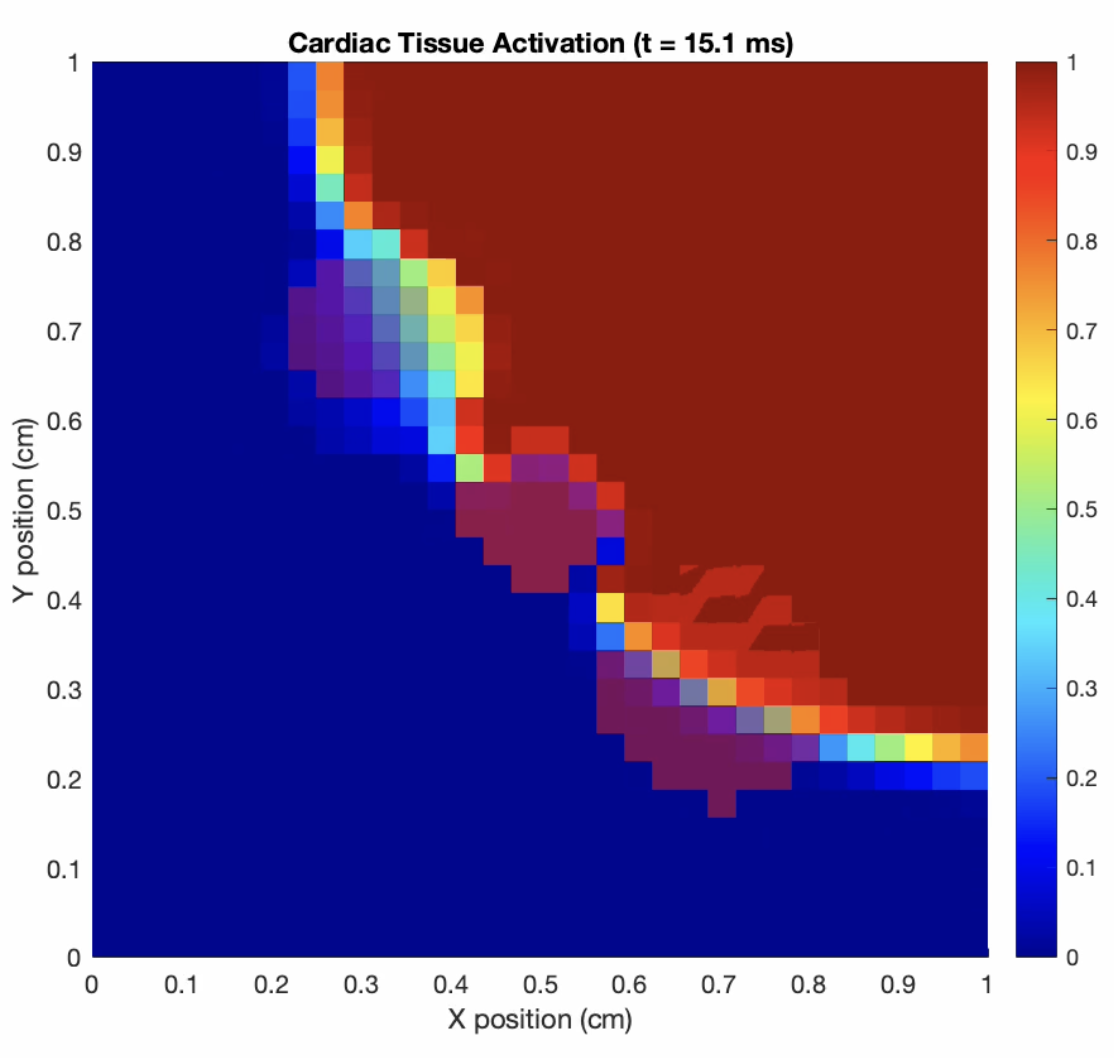
\includegraphics[width=0.7\textwidth]{../assets/images/activation_t15.png}
        \caption{Early propagation at $t=15.1$ ms}
        \label{fig:activation_t15}
    \end{subfigure}
    \hfill
    \begin{subfigure}[b]{0.48\textwidth}
        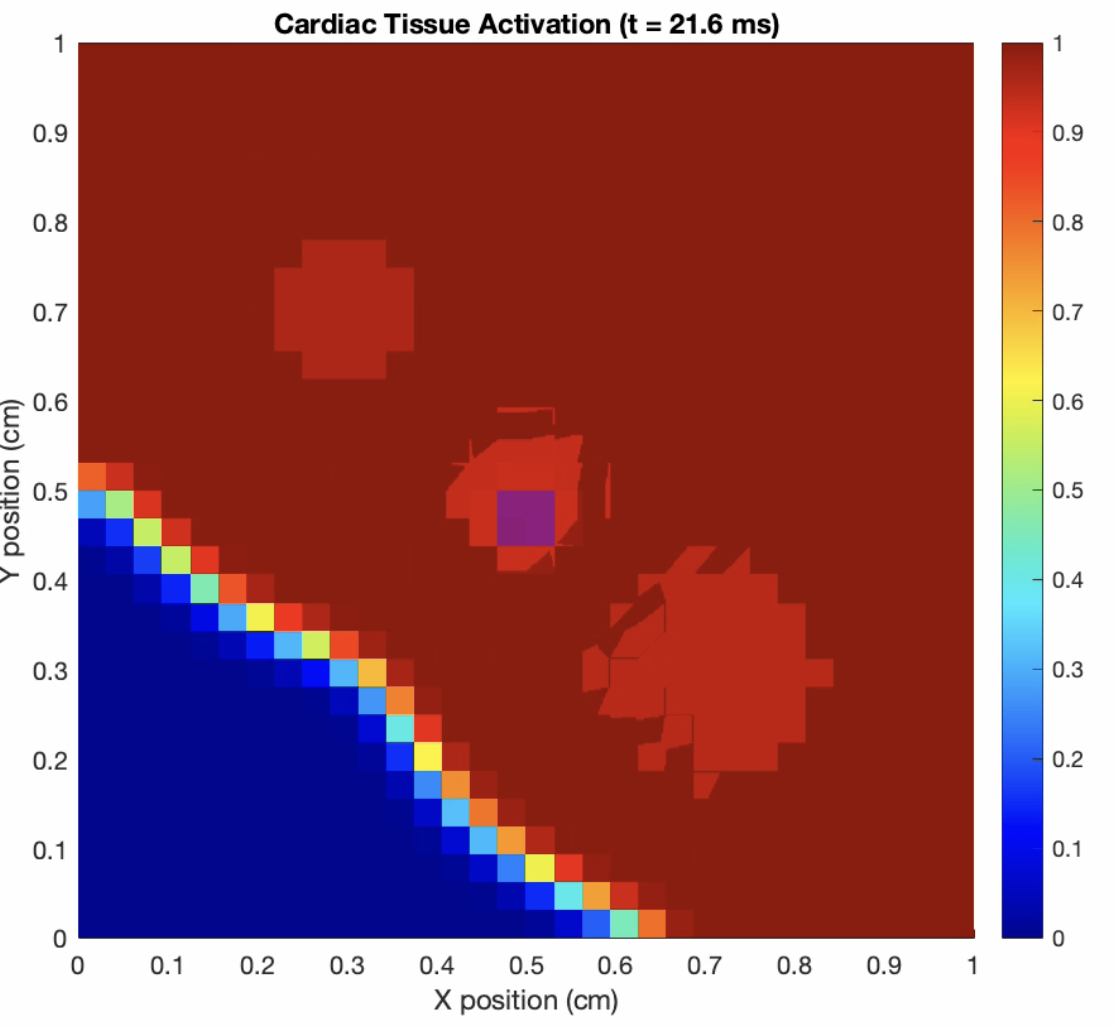
\includegraphics[width=0.7\textwidth]{../assets/images/activation_t21.png}
        \caption{Advanced propagation at $t=21.6$ ms}
        \label{fig:activation_t21}
    \end{subfigure}
    \caption{Electrical potential propagation through heterogeneous cardiac tissue. The three diseased regions $\Omega_{d1}$, $\Omega_{d2}$, and $\Omega_{d3}$ show distinct effects on wave propagation depending on their conductivity ratios.}
    \label{fig:activation}
\end{figure}

\paragraph{Propagation Dynamics Analysis}

The simulation reveals several key propagation characteristics:

\begin{itemize}
    \item \textbf{Hyper-conductive Regions} ($\sigma_d = 10\sigma_h$): Enhanced conduction velocity creates preferential pathways, leading to faster activation and potential re-entry phenomena.
    
    \item \textbf{Normal Conductivity} ($\sigma_d = \sigma_h$): Uniform wave propagation maintains circular wavefront geometry, serving as the control case.
    
    \item \textbf{Hypo-conductive Regions} ($\sigma_d = 0.1\sigma_h$): Significantly slowed conduction creates "slow zones" that can act as barriers to propagation or sources of delayed activation.
\end{itemize}

\paragraph{Clinical Relevance}
These propagation patterns have direct clinical implications:
\begin{itemize}
    \item \textbf{Arrhythmia Risk}: Regions with extreme conductivity contrasts can create conditions for re-entrant circuits
    \item \textbf{Conduction Block}: Severely hypo-conductive regions may completely block wave propagation
    \item \textbf{Activation Delay}: Heterogeneous patterns alter the synchronization of cardiac muscle contraction
\end{itemize}

\subsubsection{Quantitative Analysis}

Figure~\ref{fig:bounds-check} and Figure~\ref{fig:activation-heatmap} provide quantitative analysis of the parameter space exploration.

\begin{figure}[H]
    \centering
    \begin{minipage}{0.55\textwidth}
        \centering
        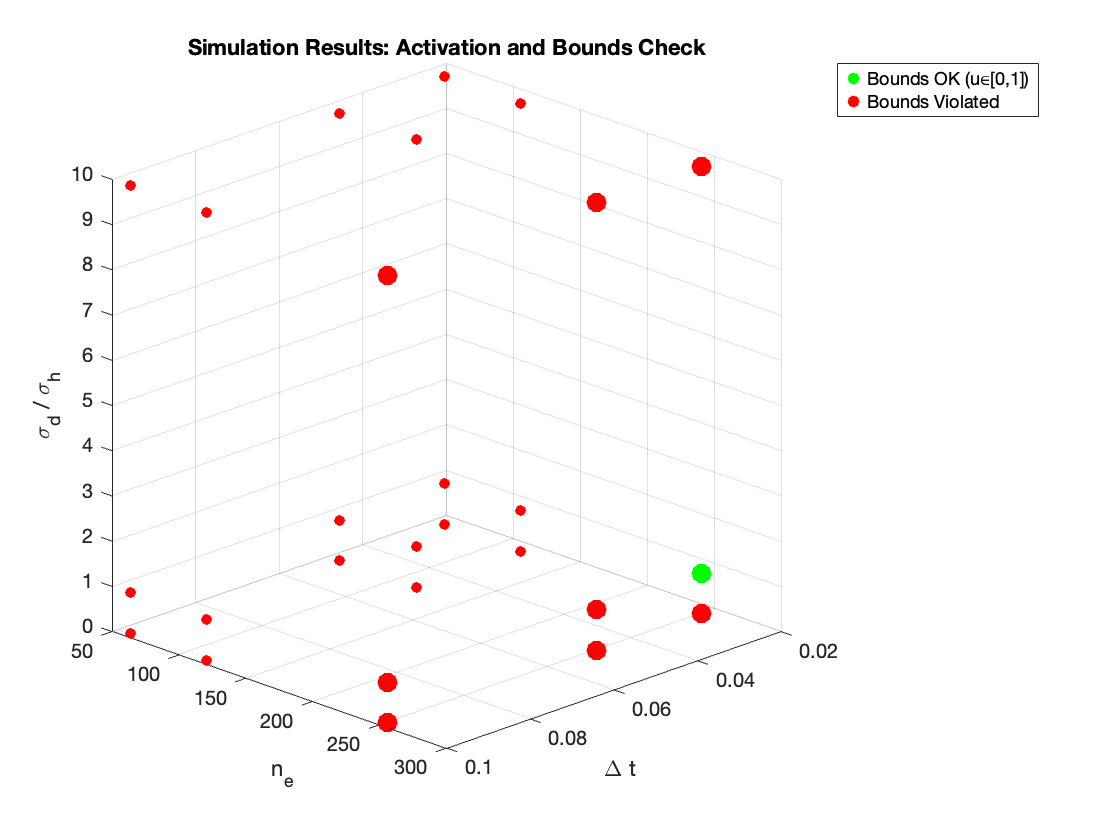
\includegraphics[width=\textwidth]{../assets/images/sim_results.png}
        \caption{3D visualization of simulation outcomes in parameter space $(\Delta t, n_e, \sigma_d/\sigma_h)$. Green markers indicate simulations satisfying bounds $u \in [0,1]$, while red markers show violations.}
        \label{fig:bounds-check}
    \end{minipage}
    \hfill
    \begin{minipage}{0.4\textwidth}
        \centering
        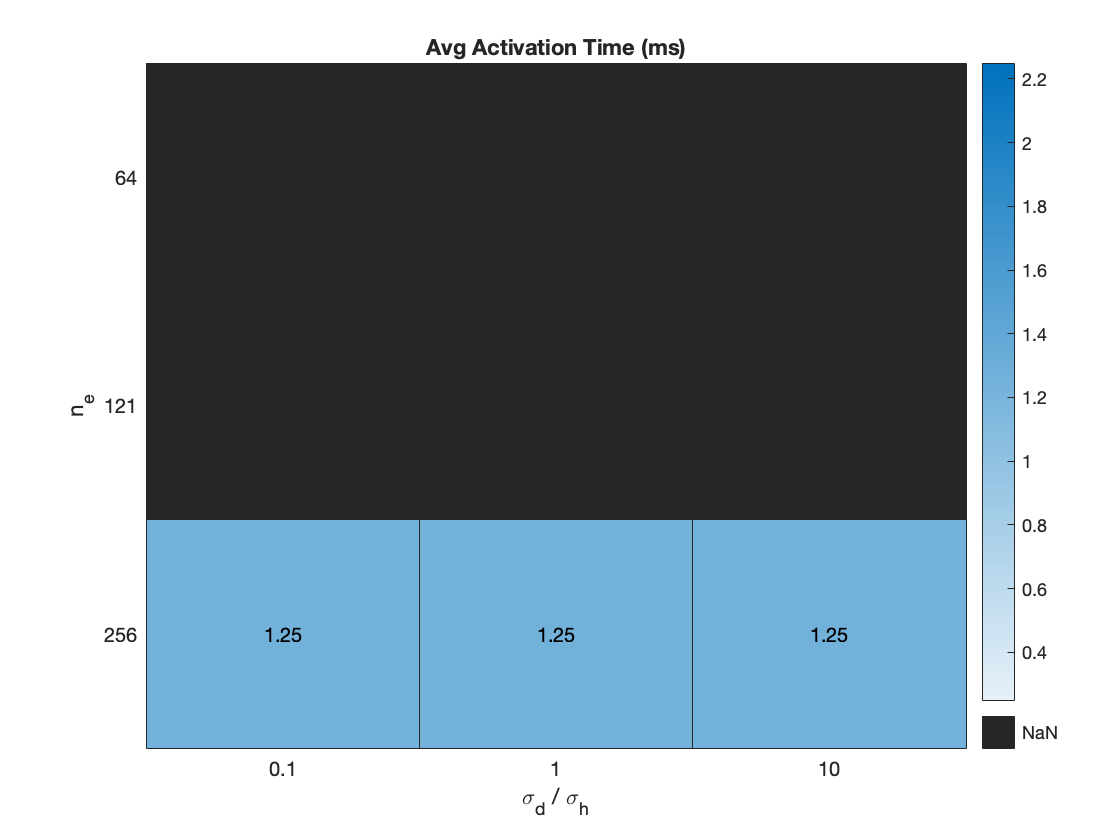
\includegraphics[width=\textwidth]{../assets/images/heatmap.png}
        \caption{Heatmap showing average activation times for valid parameter combinations. Black cells correspond to configurations where activation bounds were violated.}
        \label{fig:activation-heatmap}
    \end{minipage}
\end{figure}

The analysis reveals that successful simulations (green in Figure~\ref{fig:bounds-check}) form a very narrow region in parameter space, highlighting the delicate balance required between spatial resolution, temporal accuracy, and material heterogeneity. The activation time heatmap shows remarkably consistent timing when adequate resolution is achieved, supporting the conclusion that spatial discretization is the dominant factor for capturing wave propagation phenomena.

\subsection{Finite Element Method: Conclusions and Limitations}

\subsubsection{Strengths of the FEM Implementation}

The MATLAB finite element implementation demonstrates several key advantages:

\begin{itemize}
    \item \textbf{Structured Implementation}: The modular design with separate functions for mass and stiffness matrix assembly provides excellent code maintainability and extensibility.
    
    \item \textbf{Heterogeneity Support}: The modified assembly function elegantly handles spatially varying conductivity without compromising computational efficiency or sparsity patterns.
    
    \item \textbf{Stability Analysis}: The systematic evaluation of M-matrix properties and solution bounds provides important insights into numerical stability.
    
    \item \textbf{Comprehensive Testing}: The automated parameter sweep reveals critical dependencies and failure modes that might be missed in ad-hoc testing.
\end{itemize}

\subsubsection{Identified Limitations}

Several important limitations emerged from the analysis:

\begin{enumerate}
    \item \textbf{Resolution Requirements}: The critical dependence on fine spatial discretization ($n_e = 256$) for activation detection suggests that the method may be computationally expensive for larger domains or 3D problems.
    
    \item \textbf{M-Matrix Property}: The consistent failure to achieve M-matrix properties across all tested configurations indicates potential issues with solution positivity, particularly important for physically meaningful results.
    
    \item \textbf{Bounds Violations}: The frequent violation of solution bounds $u \in [0,1]$ suggests that the IMEX scheme may require stabilization for robust performance across diverse parameter ranges.
    
    \item \textbf{Temporal Sensitivity}: The strong coupling between spatial and temporal discretization parameters limits the flexibility in choosing efficient time step sizes.
\end{enumerate}

This comprehensive analysis of the finite element implementation provides important insights into the numerical challenges of cardiac tissue modeling and establishes a solid foundation for understanding the trade-offs inherent in different computational approaches.


\section{Deep Learning Approaches}

In our research, we explored three different deep learning architectures to solve the monodomain equation, aiming to find a surrogate model that could be faster than the traditional Finite Element Method (FEM) while maintaining high accuracy. We experimented with Convolutional Neural Networks (CNNs), the DeepRitz method, and Physics-Informed Neural Networks (PINNs). Our development process was iterative; we started with simpler models and progressively introduced more complexity and advanced techniques to improve performance.

\subsection{Convolutional Neural Network (CNN) as a Surrogate Model}

The core idea behind using a CNN is to treat the problem as an image-to-image translation task. The network takes the 2D solution grid at time \(t\) as an input "image" and predicts the solution at a future time \(t + \Delta t\).

\subsubsection{Initial Model: $cnn\_model\_000001$}
Our first attempt was a standard U-Net architecture. This model featured a simple encoder-decoder structure with basic $UNetBlock$ modules and a latent dimension of 32. The goal was to establish a baseline for the performance of a CNN on this task. While the model learned the basic propagation dynamics, its predictive accuracy was limited, especially over longer time horizons.

\begin{figure}[H]
    \centering
    
\includegraphics[width=0.8\textwidth]{../models/cnn\_model\_000001/training_loss.png}
    \caption{Training loss for the initial CNN model ($cnn\_model\_000001$).}
    \label{fig:cnn_loss_1}
\end{figure}

\subsubsection{Advanced Model: $cnn\_model\_000002$}
To improve upon the baseline, we developed a more sophisticated architecture. The key enhancements in this version were:
\begin{itemize}
    \item \textbf{Residual Connections:} We replaced the standard U-Net blocks with $ResUNetBlock$s. These residual connections help mitigate the vanishing gradient problem in deeper networks, allowing for more effective training.
    \item \textbf{Increased Depth and Latent Space:} We significantly deepened the encoder and decoder and increased the latent dimension to 128, allowing the model to capture more complex spatial features.
    \item \textbf{Regularization:} We introduced Dropout with a rate of 0.2 to combat overfitting.
\end{itemize}
This model ($cnn\_model\_180652$, saved as $cnn\_model\_000002$) was trained for 1000 epochs, achieving a final training loss of 0.04 and a validation loss of 0.32. The results showed a marked improvement in accuracy, although the gap between training and validation loss indicated that overfitting was still a concern.

\begin{figure}[H]
    \centering
    
\includegraphics[width=0.8\textwidth]{../models/cnn\_model\_000002/training_loss.png}
    \caption{Training and validation loss for the advanced ResUNet model ($cnn\_model\_000002$).}
    \label{fig:cnn_loss_2}
\end{figure}

\subsubsection{Further Experiments: $cnn\_model\_010647$ and $cnn\_model\_104653$}
In subsequent iterations, we experimented with state-of-the-art techniques to further enhance training stability and generalization:
\begin{itemize}
    \item \textbf{Weight Standardization and Spectral Normalization:} These techniques were introduced to regularize the weights of the convolutional layers, improving the conditioning of the optimization problem.
    \item \textbf{Group Normalization:} We replaced Batch Normalization with Group Normalization to make the training process less dependent on the batch size.
    \item \textbf{Stochastic Depth:} During training, entire ResUNet blocks were randomly dropped. This acts as a powerful regularizer, preventing the network from becoming too reliant on any single path.
\end{itemize}
These advanced models demonstrated more stable training dynamics, but required careful hyperparameter tuning. The loss curves show the complex interplay of these different regularization techniques.

\begin{figure}[H]
    \centering
    \begin{subfigure}[b]{0.48\textwidth}
        
\includegraphics[width=\textwidth]{../models/cnn\_model\_010647/training_loss.png}
        \caption{Model $cnn\_model\_010647$}
        \label{fig:cnn_loss_3}
    \end{subfigure}
    \hfill
    \begin{subfigure}[b]{0.48\textwidth}
        
\includegraphics[width=\textwidth]{../models/cnn\_model\_104653/training_loss.png}
        \caption{Model $cnn\_model\_104653$}
        \label{fig:cnn_loss_4}
    \end{subfigure}
    \caption{Training losses for CNNs with advanced regularization techniques.}
\end{figure}

\subsection{Deep Ritz Method}
The Deep Ritz method offers a different paradigm. Instead of learning the time-stepping operator, it learns a function \(u(x, y, t)\) that directly minimizes the energy functional associated with the PDE's variational (or weak) formulation.

\subsubsection{Model $deepritz\_model\_220842$}
Our implementation, $DeepRitzSolver$, is a Multi-Layer Perceptron (MLP) that takes spatial and temporal coordinates \((x, y, t)\) as input and outputs the solution \(u\). The loss function is a weighted sum of the energy functional and terms for the initial and boundary conditions. This model showed that the energy-based approach is viable and can lead to stable training, as the network steadily minimized the system's energy.

\begin{figure}[H]
    \centering
    
\includegraphics[width=0.8\textwidth]{../models/deepritz\_model\_220842/training_loss.png}
    \caption{Training loss for the Deep Ritz model ($deepritz\_model\_220842$).}
    \label{fig:deepritz_loss}
\end{figure}

\subsection{Physics-Informed Neural Network (PINN)}
The PINN approach is similar to Deep Ritz in that it learns the function \(u(x, y, t)\), but it enforces the PDE in its strong form. The loss function directly penalizes the PDE residual.

\subsubsection{Model $pinn\_model\_113908$}
Our $PINNSolver$ uses an MLP architecture similar to the Deep Ritz model. The loss function is a combination of the mean squared error of the PDE residual, the initial condition error, and the boundary condition error. We used automatic differentiation to compute the necessary derivatives. Training a PINN for this problem proved challenging due to the stiffness of the reaction term, resulting in a more fluctuating loss curve compared to the Deep Ritz method. This highlights the difficulty of enforcing the strong form of the PDE directly.

\begin{figure}[H]
    \centering
    
\includegraphics[width=0.8\textwidth]{../models/pinn\_model\_113908/training_loss.png}
    \caption{Training loss for the PINN model ($pinn\_model\_113908$).}
    \label{fig:pinn_loss}
\end{figure}

\end{document}
